\documentclass[tikz,border=10pt]{standalone}
\usepackage{amsmath}
\usepackage{tikz}
\usetikzlibrary{arrows.meta, positioning, angles, quotes, decorations.markings, calc}

\begin{document}

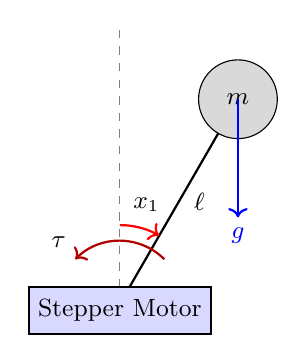
\begin{tikzpicture}[
  mass/.style = {circle, draw, fill=gray!30, minimum size=1cm},
  string/.style = {thick},
  anglemark/.style = {draw, ->, thick, red},
  force/.style = {->, thick, blue},
  arrow/.style = {thick, -{Latex[width=2mm]}},
  torque/.style = {->, thick, red!70!black},  
  motor/.style = {draw, thick, rectangle, fill=blue!15, minimum width=1cm, minimum height=0.6cm},
  every node/.style = {font=\small}
]

% Parameters
\def\L{3}
\def\theta{30} % degrees

% Coordinates
\coordinate (pivot) at (0,0);
\coordinate (bob) at ($(pivot) + ({90 - \theta}:\L)$);  % now inverted
\coordinate (equilibrium) at ($(pivot) + (90:\L)$);

% Draw dashed vertical equilibrium line
\draw[dashed, gray] (pivot) -- ++(90:\L+0.5);

% Draw the pendulum
\draw[string] (pivot) -- (bob);
\node[mass] at (bob) {$m$};

% Draw pivot
\filldraw[black] (pivot) circle (2pt);

% Angle arc from vertical to pendulum line (90° to 90 - θ)
\draw[anglemark] (pivot) ++(90:1) arc[start angle=90, end angle={90 - \theta}, radius=1];
\node at ($(pivot)+({90 - 0.5*\theta}:1.3)$) {$x_1$};


% Gravity force
\draw[force] (bob) -- ++(0,-1.5) node[below] {$g$};

% Length label
\path (pivot) -- node[midway, right=2pt] {$\ell$} (bob);

% External torque at pivot (counterclockwise arrow)
% External torque at pivot (counterclockwise arrow)
\draw[torque] ([shift=(45:0.8cm)]pivot) arc[start angle=45, end angle=135, radius=0.8];
\node at ($(pivot)+(135:1.1)$) {$\tau$};
 
% Stepper motor at pivot
\node[motor, anchor=south] at ($(pivot)+(270:0.4)$) {Stepper Motor};

\end{tikzpicture}

\end{document}
